\section*{Problem}
From user feedback of the Faroese statbank, we know that the Faroese statbank has lots of usability issues.

The UI\footnote{User Interface\label{t::ui}} is not up to date with modern web standards and it does not contain any responsive modules, like visualization of the data. The UI is also legacy code\footnote{ code without tests, which reflects the perspective of legacy code being difficult to work with in part due to a lack of automated regression tests}. 

This is a cross national problem since users in several countries, including all the Nordic countries, are facing the same usability problems.

\begin{figure}[H]
  \centering
  \begin{subfigure}[b]{0.3\linewidth}
    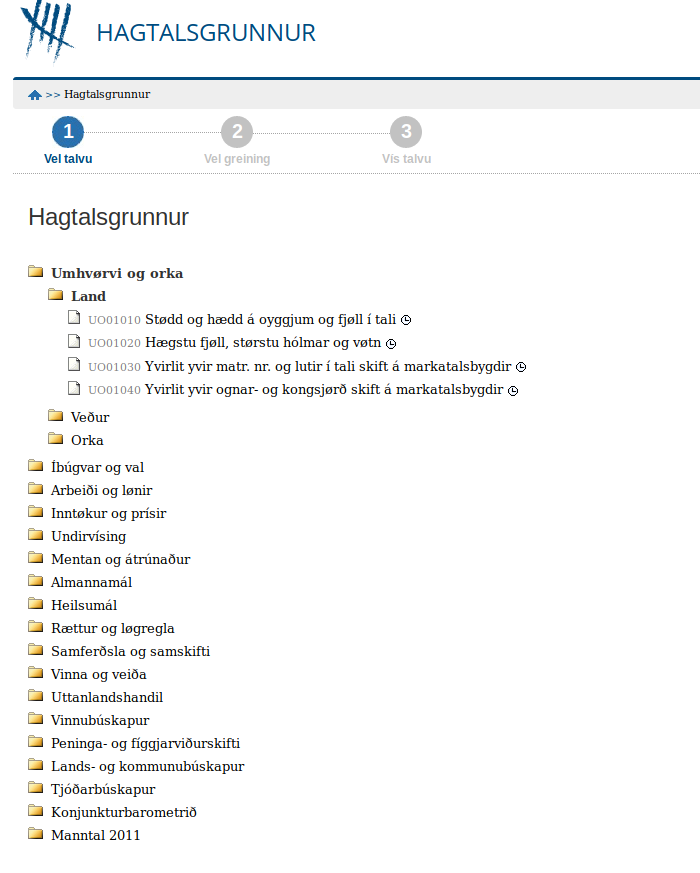
\includegraphics[width=\linewidth]{img/ui1.png}
    \caption{List}
    \label{fig:List}
    
  \end{subfigure}  
  \begin{subfigure}[b]{0.3\linewidth}
    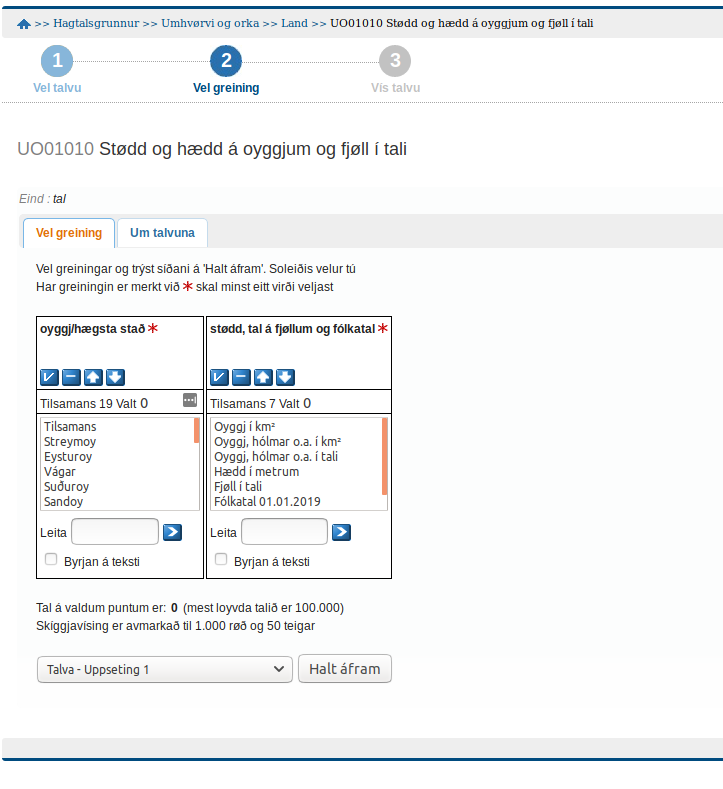
\includegraphics[width=\linewidth]{img/ui2.png}
    \caption{Selectors}
    \label{fig:selectors}
    
  \end{subfigure}  
  \begin{subfigure}[b]{0.3\linewidth}
    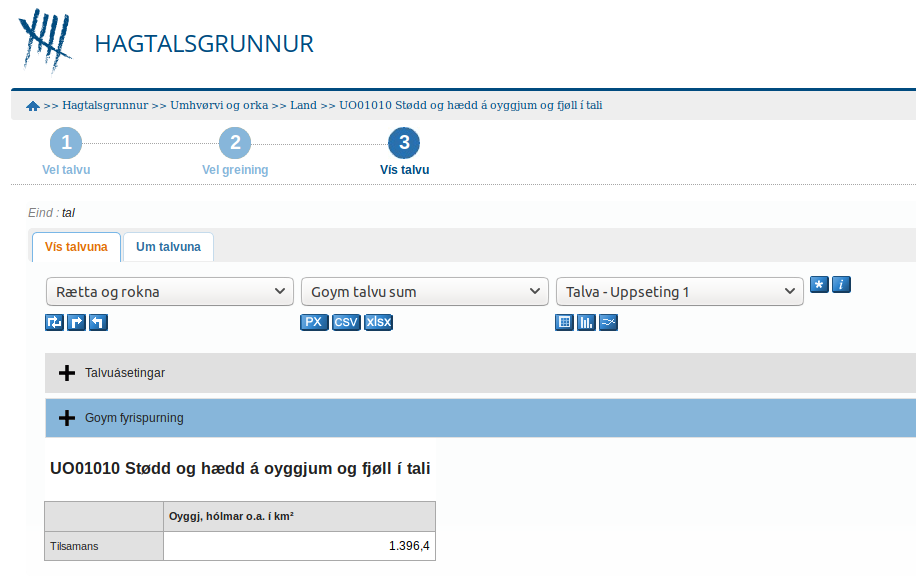
\includegraphics[width=\linewidth]{img/ui3.png}
    \caption{Result}
    \label{fig:result}
    
  \end{subfigure}  
  \caption{User Interface (Faroese Statbank)}
  \label{fig:uifaroesestatsbank}
\end{figure}

If we start with figure1\ref{fig:uifaroesestatsbank}, we can see that the UI is not up to standard with modern web applications. The UI needs a new modern look.

As it is now, the user has to go through $3$ pages to get to the result. This should be unnecessary. So to give the user a better experience, all $3$ pages should be fit on $1$ page.

\noindent\fbox{%
    \parbox{\textwidth}{%
\begin{description}
\item [List\ref{fig:List}] The structure of the list is good and simple to understand. The real change here is to give it a modern style and try to make it more responsive.

\item [Selectors\ref{fig:selectors}] The Selectors need a new styling and new functionality that give the user a instant result\ref{fig:result} response. This means that the result changes when a selector changes.

\item [Result\ref{fig:result}] The results only need new styling since the functionality of results is good. 

\end{description}
    }%
}




  
\section{Complex of unsolved problems}
How can we utilize the API with modern web components, to improve the user experience and even rethink the way how it can be used.

\section{Aim of project}
The aim of the project is to build a new modern responsive UI prototype of the Faroese statbank as a concept.

If the project is a success, the concept will shown at the yearly $PXWEB$ conference\footnote{held in Nov 2019 in Armenia}, to show the other statistic organizations how $PXWEB$ can be utilized with modern components and not least give them inspiration of recreating their own modern statbank UI with this prototype as a template and share their experience. 

\section{Technology}
To make the prototype a reality I will be using $JavaScript$ as the main programming language. $JavaScript$ is one of the worlds most used front-end programming language\footnote{\href{http://blog.stoneriverelearning.com/top-10-programming-languages-used-in-web-development/}{Top 10 programming languages used in web development}\label{jstop10}}. Addition to this, I will be using the $React$\footnote{\href{https://reactjs.org/}{Reactjs}\label{react}} library for building the user interface. $React$ main maintainer is Facebook.

$Material-UI$\footnote{\href{https://material-ui.com/}{Material-ui}\label{mui}} will also be used for the design.$Material-UI$ is a popular $React$ UI Framework. 

$TypeScript$\footnote{\href{https://www.typescriptlang.org/}{TypeScript}\label{typeScript}} is also being considered.

$TypeScript$ is a strongly typed, object oriented, compiled language. It was designed by Anders Hejlsberg at Microsoft. $TypeScript$ is both a language and a set of tools. $TypeScript$ is a typed superset of $JavaScript$ compiled to JavaScript. In other words, $TypeScript$ is $JavaScript$ plus some additional features\footnote{\href{https://www.tutorialspoint.com/typescript/typescript_overview}{What is TypeScript}\label{whatIsTypeScript?}}.

Other programming languages where also considered:
\begin{description}

\item [.Net\footnote{\href{https://dotnet.microsoft.com/}{.NET}\label{.net}}] Is a really good platform, but I find it best to use when working with databases and applications that use CRUD\footnote{Create,read,update,delete}. For example, a online store or accounting.
\item [R Shiny\footnote{\href{https://www.rstudio.com/products/shiny/}{R Shiny}\label{rShiny}}] The package $R Shiny$ looks really interesting for visualizing data, but since one of the aims of the project is to give other statistic organizations inspiration of recreating their own modern statbank UI with this prototype as a template and share their experience. The best way forward is to use $JavaScript$ that is probably worlds most used front-end programming language. 
\end{description}


